\chapter{Assembly and Dynamics of Rod-Shaped Colloids}
\label{ch:rods}
\section{Introduction}

When one is first presented with the different dimensions of anisotropy proposed by 
Glotzer and Solomon (Figure~\ref{fig:glotzer-dimensions},~\cite{glotzer-solomon}), the
potential variety of particle types can be overwhelming. It is therefore useful to begin by studying 
particles which draw from only one or two of these anisotropy dimensions. To this end, our
initial study has focused on particles which vary only in the dimension of 
aspect ratio, i.e. colloidal rods. This study covers the fabrication of both single-component and 
Janus rods by stop-flow lithography, the study of rod diffusion by particle tracking, and the basics
of self-assembly for Janus rods in different solvents.

In Section~\ref{sec:rods-background}, the flow lithography technique for particle microfabrication
is described in detail. Section~\ref{sec:rods-exp} describes the experimental procedure for 
the fabrication of SFL microfluidic devices, the fabrication of single-component and Janus rods,
particle collection and purification
and the observation of rod suspensions by fluorescence and confocal microscopy. 
Section~\ref{sec:rod-collection} describes the results of trials on different rod collection
techniques, while Section~\ref{sec:surface-interact} describes observations of 
surface interactions between colloidal rods and various surfaces. Section~\ref{sec:rod-diffusion-results}
shows the results of translational and rotational diffusion measurements, and 
Section~\ref{sec:assembly-janus-rods} describes experiments on the 
self-assembly of Janus rods.

%%%%%%%%%%%%%%%%%%%%%%%%%%%%%%%%%%%%%%%%%%%%%%%%%%%%%%%%%%%%%%%%%%%%%%%%%%%%%%%%%%%%%%%%%%%%%%%
\section{Background}
\label{sec:rods-background}

\subsection{Continuous-Flow Lithography}

One method for the fabrication of structured particles which has undergone active development in recent years is 
\textit{flow lithography}, a technique developed by Patrick Doyle at MIT which combines microfluidics with 
UV lithography.  Flow lithography may be carried out either in a continuous-flow mode or in a 
mode where flow is stopped for the photopolymerization step.

\figone{fig:sfl-schematic}{figures/literature-review/doyle-sfl-schematic.png}{\linewidth}{
Schematic of stop-flow lithography experiment.~\cite{dendukuri-sfl}}

\figone{fig:sfl-o2-inhib}{figures/literature-review/doyle-sfl-o2-inhibition.png}{\linewidth}{
Oxygen inhibition of photopolymerization in a PDMS microfluidic device.~\cite{dendukuri-oxygen}}

In a typical continuous flow lithography experiment,~\cite{dendukuri-cfl},
we construct a microfluidic device out of polydimethylsiloxane (PDMS)
which contains a simple straight microchannel with cross-sectional dimensions between 5-400 \microns. As a feedstock
material we use some fast-photocuring low-viscosity liquid, typically a photocurable monomer solution. The device is 
placed on a microscope which includes some UV illumination source which may be reversed through the optical path (i.e.
it is emitted at the objective lens) and a fast electronic shutter. A typical example might be a conventional 
fluorescence microscope with a mercury lamp.  A
transparency photomask defining the particle geometry is placed at the microscope
field stop to mask the UV beam.
To fabricate particles, the photocurable liquid is pumped 
at a constant rate through the microchannel, and the microchannel is oriented
parallel to the microscope's focal plane. The microscope objective is focused on a plane inside the channel
volume, and the
electronic shutter is opened at intervals. If the UV light is intense enough and the liquid is moving at a slow enough speed,
the UV-exposed region will cure into one or more solid particles.  
The microchannel flow carries these particles out of the ``active 
region'', and provides fresh material.

The particle geometry is defined by a combination of the photomask and the microchannel.  The two-dimensional cross-section
is determined by the shape of the UV beam at its intersection with the microchannel, and the particle height is defined by
the height of the microchannel. The upper and lower surfaces of the particles
are flat, as they conform to the upper and lower microchannel surfaces, so that the particle geometry
is a 3D extrusion of the photomask.
Friction or sticking with these top and bottom
surfaces are prevented in the case where PDMS is the channel material and a hydrogel monomer is the feedstock: hydrogel
curing is inhibited by the presence of oxygen, and PDMS is oxygen permeable. This results in the formation of an 
``inhibition layer'' along the internal surfaces of the channel where the liquid will not cure, preserving the mobility 
of the particles (see Figure~\ref{sfl-o2-inhib}).~\cite{dendukuri-oxygen}
This layer is typically a few microns thick, depending on 
details of the channel construction.
The resolution and quality of the 2D pattern 
is affected by the quality of focus, the resolution of the mask,
and the magnification and numerical aperture of the objective lens.  

\subsection{Stop-Flow Lithography}
\label{sec:SFL}

In \textit{stop-flow lithography} (SFL), the cure-during-flow
procedure in continuous flow lithography is replaced with a flow-stop-cure cycle in which the microchannel flow
is allowed to come to a halt before UV exposure. This change allows for a substantial improvement in both 
fabrication resolution and throughput.~\cite{dendukuri-sfl}

First, resolution is improved because stopping the microchannel flow minimizes the effect of polymerization
``smearing'', which distorts the shape of the resulting particles.
When flowing monomer solution is exposed to UV light for some finite time, any monomer which occupies the exposed volume 
during that time begins to undergo photo-polymerization.  Some of the solution will flow out of this region 
during this time, and be replaced by additional solution from up-stream. This results in a particle which is ``smeared''
or ``stretched'' along the direction of flow, and does not precisely reproduce the shape defined on the mask.  
When flow is 
stopped, this effect is minimized, and the only limitations imposed on the resolution are due to the optical system,
the mask resolution and materials constraints.

Second, throughput is greatly increased because higher rates of flow may be used during the periods when pressure is
applied.  In continuous-flow lithography, the rate of flow must be kept relatively slow to allow curing to take place
at all.
Once particles have cured, no 
additional exposure step may take place until this flow has carried the particles out of the
exposure region and fresh monomer has been supplied to carry out another cure step.  In SFL, the rate of flow
between exposure steps
may be arbitrarily high as the cure step is carried out when the flow is stopped. 
When the cure step is finished in SFL, a high pressure is applied to quickly clear the exposure region, followed by a 
short pause to allow the fluid to stop flowing.  This procedure has allowed fabrication rates as high as 
$10^5$ particles min$^{-1}$.~\cite{dendukuri-sfl}

Note that the advantage in throughput is reduced somewhat when the experiment design necessitates a long pause step
after the flow. The length of this pause step is dependent on the fluid viscosity, but especially on the 
response time of the PDMS device.  When a high pressure is applied to elastic PDMS microchannel, the 
walls of the channel deform to allow it to expand.  Removing that pressure, as in SFL, produces a ``squeeze flow''
phenomenon in which the relaxation of the device walls generates some fluid flow within the channel. The cure step 
cannot take place until this flow has ceased.  This response time may be given as

\begin{equation}
\tau_r \sim \frac{\mu L^2 W}{EH^3}
\end{equation}

where $L$ is the channel length, $W$ is the channel width, $H$ is the channel height and $E$ is the elastic
modulus of PDMS.  Note that this response time is not dependent on the input pressure, so that relatively high
flow rates may be used without affecting the length of the pause step. However, this scaling becomes pressure-dependent
and more complicated when the deformation in channel height $\Delta h$ is comparable to $H$.~\cite{dendukuri-sfl}

\subsection{Multiple-Component Fabrication}

Polymeric particles consisting of multiple components of different chemistries may be produced by taking advantage
of laminar flow in the fabrication microchannel.  
In the laminar flow regime, several different streams may flow in parallel through
the same microchannel without turbulence, with mixing limited to that caused by 
diffusion.~\cite{stone-laminar}  Diffusion alone
will produce very little mixing, so that a sharp boundary between two streams may spread only a few microns over
millimeters of linear flow.~\cite{mohr-flow} The result is a multiple-stream microchannel flow in which multiple materials
co-exist and are geometrically distinct.

If each co-flowing stream is made up of a photopolymerizable solution with similar curing kinetics, one may perform
flow lithography using a mask which illuminates several streams at once to produce particles which contain geometrically
distinct regions of different chemical makeup.  A simple case 
is demonstrated in Dendukuri \textit{et al.}~\cite{dendukuri-sfl}
for SFL, in which dyed and un-dyed PEGDA solutions are cured in the laminar flow regime to produce particles whose
fluorescence is confined to one part of the particle.  Fabrication of amphiphilic microparticles containing both
hydrophobic and hydrophilic materials is demonstrated in another Dendukuri paper in 
\textit{Langmuir}~\cite{dendukuri-amph}, and particles which incorporate biomolecule probes and lithographically-defined
``barcodes'' in different regions are fabricated by Pregibon \textit{et al.} in a 2007 paper in 
\textit{Science}.~\cite{pregibon-dna}

\section{Experimental Procedure}
\label{sec:rods-exp}

Colloidal rods were fabricated by stop-flow lithography (SFL) as described in Section~\ref{sec:SFL} using
hydrophobic and hydrophilic monomer solutions.  

\subsection{Microchannel Device Fabrication}

\figone{fig:device-design}{figures/rods/four-channels-together.jpg}{0.5\linewidth}{
Four Y-channel microchannel patterns, sharing a common reservoir for accumulation of particles from multiple experiments.}

Particle fabrication was carried out in 
three-input Y-junction microchannel devices (Figure~\ref{fig:device-design}).
The primary channel of these devices had a typical 
height of 7 \microns, width of 200 \microns, and length of 3000-5000 \microns. These dimensions were selected
to facilitate the fabrication of large numbers of particles with small size in all dimensions: the low height
facilitated small-particle fabrication by limiting the height of the particles, while the comparatively large
width allowed many particles to be fabricated simultaneously. Multiple inputs were included to allow up to three
monomer streams to be simultaneously flowed, with a single exit point for collecting particles.

\subsubsection{Photoresist Masters}
Positive-relief photoresist master templates were fabricated by UV photolithography. A thin film
of SU-8 2007 photoresist (Microchem) was laid down on a clean Si wafer by spin-coating at 3000 rpm to produce a 
7 \microns~layer. Next, a ``soft bake'' was carried out by heating the wafer on a hot plate at 
120\degC~for five minutes to evaporate the photoresist solvent.  The device features were patterned by exposing the 
photoresist to UV light from a 300 W lamp for 40 s through a photomask defining the device design. A ``hard bake'' step
was then carried out by heating the wafer at 120\degC for ten minutes, to cure the photoresist in the exposed areas.
Finally, the wafer was immersed in SU-8 developer (Microchem) and agitated for two minutes to remove the unexposed
photoresist, then rinsed with isopropyl alcohol (IPA).

After fabrication, photoresist masters were subjected to a fluorinated silane vapor coating to inhibit adhesion
between the SU-8 template and the elastomer to be cast. Masters were placed in a small desiccator (Fisher Scientific)
along with an open container of (tridecafluoro-1,1,2,2-tetrahydrooctyl) trichlorosilane (``fluorosilane'', Gelest, Inc.)
This desiccator's vacuum port was then connected to a single-stage vacuum pump 
(Fisher Scientific) and evacuated for two hours to produce
a silane coating.

\subsubsection{Elastomer Device Construction}

Microchannel devices were constructed from polydimethylsiloxane (PDMS, Dow Corning, Sylgard 184). PDMS
elastomer and curing agent were mixed at a ratio of 10:1 by weight, and pored over the photoresist master 
in a plastic petri dish to a depth of about 2 mm.  PDMS was also spun-coat onto a 48 x 60 mm \#1 cover-slip (Gold Seal)
to form the substrate for the device.
Both of these  were then baked at 65\degC~for six hours or more to cure
the PDMS.  

Once the PDMS was fully cured, a razor blade was used to carefully cut out a section which encompassed some or all of
the microchannels defined on the photoresist master. This section was then peeled up from the master, resulting
in a block of PDMS with negative features defining the tops and sides of the microchannels.
For each microchannel, three small holes ($\sim$0.5 mm) were punched at each entrance using a syringe press, and a larger
hole ($\sim$3 mm) was punched at the exit using a biopsy punch.

For each of the ``top side'' PDMS block and the PDMS-coated glass substrate, the PDMS surface was rinsed with 
deionized water and IPA.  Following this, small particles were removed by first laying down and then peeling up
Scotch Magic brand transparent tape.  Each section was then placed below a UV light-emitting
tube lamp with the channel surface facing the lamp, and exposed to UV light for ten minutes to promote PDMS-PDMS
adhesion.  After UV exposure, the channels and the 
substrate were then firmly pressed together with the channel surface of the top
block against the PDMS-coated surface of the substrate.  The resulting device was then baked at 100\degC~for one hour
to promote device bonding.

\subsection{Photocurable Solutions}
\label{sec:janus-materials}
The hydrophobic solution was composed of 95 v/o 
tri(methylol propane) triacrylate (TMPTA, Sartomer) and 5 v/o Darocur 1173 photoinitiator (Ciba), 
with 0.005 wt\% methacryloxyethyl thiocarbamoyl rhodamine B (Polysciences) as a cross-linking 
fluorescent dye.
The hydrophilic solution was composed of either 20 mol ethoxylated tri(methylol propane) triacrylate (20-ETMPTA,
Sartomer) or poly(ethylene glycol) diacrylate (PEGDA, $M_n$ = 700, Sigma Aldrich) at 80 v/o, 
15 v/o deionized water, and 5 v/o Darocur 1173 photoinitiator, with 0.005 wt\% 
3,8-dimethacryloyl ethidium bromide (Polysciences) as a cross-linking fluorescent dye.


\subsection{Mask Design}

Masks used for single-component fabrication contained two-dimensional arrays of identical aligned 
rods, with a separation in each direction equal to twice the length of the rod to avoid inter-particle
curing (Figure~\ref{fig:rod-masks}(a)). These arrays were designed to maximize the number of 
rods cured per cycle by making them large enough to, at minimum,
cover the field stop aperture for the transmission of the UV beam. This circular aperture 
had a diameter of 1.5 inches.  For example, the photomask containing 500 \microns~rod features
was a twenty-by-twenty array, with the 1 mm separation ensuring that the mask area was large enough to
use the full available UV beam.  
Masks used for Janus fabrication contained only a single line of rod features, with the rods parallel to one 
another and aligned perpendicular to the axis of the line.  Spacing on these 
masks was the same as for single-component fabrication.


\subsection{SFL Experiment}
\label{sec:sfl-expt-rods}

\figone{fig:sfl-experiment-photo}{figures/rods/SFL-photo-alternate.jpg}{0.6\linewidth}{
A microfluidic device platform containing multiple Y-junction microchannels is placed on 
the microscope used for SFL, and connected to two pressure sources to pump PEGDA and TMPTA 
monomer solutions.}

%\figone{fig:sfl-schematic}{figures/literature-review/doyle-sfl-schematic.png}{0.8\linewidth}{
%General schematic of SFL experiment, illustrating computer-controlled operation of the pressure source,
%three-way valve and shutter to control flow and exposure conditions. Figure from~\cite{dendukuri-sfl}}

\figone{fig:janus-sfl-schematic}{figures/rods/janus-rod-sfl-schematic.png}{0.70\linewidth}{
SFL fabrication of Janus rods.}

UV exposure and experimental imaging for small-rod fabrication was carried out using a 60x 
oil-immersion objective lens 
on an IX72 inverted microscope(Olympus America), with an additional 1.6x lens added to the beam path for
the fabrication of smaller rods.  Using the 60x objective, a demagnification factor of approximately 
33 was typically observed between the mask and the resulting rods; i.e., a rod of 500 \microns~length defined on
the photomask would typically result in the fabrication of a 12 \microns~rod in the microchannel.

Microchannel flow was driven by gas pressure supplied by a house nitrogen line and/or a compressed air tank 
(SJ Smith Welding Supply). Pressure control was achieved using a custom-built pressure box, consisting of
four computer-controlled regulators and four duplex valves connected to a USB
controller (National Instruments) allowing for 
up to four independent pressure
settings driving up to eight separate valves. UV light was supplied by a 100 W mercury lamp
connected in fluorescence microscope configuration, with exposure time controlled using a Lambda SC 
electronic shutter (Sutter Instruments).

The SFL experiment was driven using LabView software (National Instruments) with a custom
interface. The process
flow of an SFL experiment consists of the following sequence of steps:

\begin{enumerate}
\item Specify ``flow time'' $t_{flow}$, ``pause time'' $t_{pause}$, and exposure time $t_{expose}$.
\item Set pressure for each port on electronic regulators.
\item Until the experiment is stopped:
\begin{enumerate}
\item Open valves. Wait $t_{flow}$.
\item Close valves. Wait $t_{pause}$.
\item Open shutter. Wait $t_{expose}$.
\item Close shutter. Repeat.
\end{enumerate}
\end{enumerate}

For a schematic of the SFL experimental setup, see Figure~\ref{fig:sfl-schematic}.
For each monomer solution, a 10-100\uL~pipette tip (Eppendorf) was filled with approximately 60\uL~of solution.
A silicone tube was connected at one end to the output of one valve of the pressure box, and the other end
was inserted into the top of the pipette tip.  The bottom of the pipette tip was then inserted into one of the
small entrance holes in the microchannel device.  This device was the placed on above the microscope objective,
and the microscope was focused such that the focal place was inside the channel.  After starting the 
experiment, the shutter was allowed to open and the fine focus was adjusted manually to optimize
curing conditions. Optimization was judged by visual inspection of the resulting particles. 

Single-component rods were fabricated using the central entrance channel to supply monomer to the system, 
leaving the other two entrances unused. Typical experimental settings for these experiments were pressure
8 psi, flow time 1.5 s, and pause time 2 s.  Exposure times for PEGDA or 20-ETMPTA were typically 0.05-0.15 s
depending on the mask dimensions, while exposure times for TMPTA were typically 0.2-0.3 s to compensate for
the less favorable curing behavior of the hydrophobic monomer.  The fabrication of smaller rods generally
necessitated slightly higher exposure times.  

Janus rods were fabricated using the two side entrance channels to supply each type of monomer solution,
with the central channel left unused.  (All three channels were used for fabricating
particles with complex anisotropy; see
section~\ref{sec:SFLx3}.)  Typical experimental settings for these experiments were pressure 7 psi on each side, 
flow time 2 s, pause time 2 s, and exposure time 0.2-0.3 s depending on the mask dimensions.
The two monomer streams would enter the main channel on either side, and form
an interface along the center of the channel. Because the hydrophobic and
hydrophilic streams were immiscible and the microchannel flow took place in the laminar flow regime, 
this interface persisted for several hundred microns down the channel.
During fabrication, the curing regions would be aligned such that each rod straddled this interface,
producing rods which incorporated both materials.

In either case, the resulting particles were ejected at the end of the experiment into the final reservoir, which
was left empty to allow collection of the maximum volume of particles possible.

\subsection{Particle Collection and Purification}
\label{sec:exp-collection}

Particle collection techniques were developed and optimized for a number of different experimental cases,
depending both on the particular monomer solutions involved and on the desired final rod behavior, i.e. 
non-interacting or self-assembling.  Details of the differences
in collection techniques and their effectiveness will be explored in Section~\ref{sec:rod-collection}.

In general, SFL-fabricated rods were ejected, still in monomer solution, from the fabrication microchannel into 
an open reservoir, with the bottom and sides formed of PDMS and the top open to the environment.  Owing to the
surface tension of the monomer, these particles generally stayed near the side walls of the reservoir, often
collecting in corners or imperfections of the walls.  Note that in the single-component case, the particles in
the reservoir may be assumed to be perfectly non-interacting as they are still suspended in the monomer solution, 
a solvent with the
same composition as the particles.   In the case of Janus rods this assumption is not necessarily valid, as
the particles are suspended in a mixture of the two different monomer solutions.  Once fabrication 
was complete, the collection procedure generally consisted of the following steps:

\begin{enumerate}
\item A collection solvent was introduced into the reservoir via the top opening, with volume sufficient to
fill the reservoir (generally $\sim$ 20\uL).
\item A slight delay was allowed for the particles to disperse into the new solvent from their 
original position along the 
walls. This delay was not well-controlled, but was generally between 30 and 120 s.
\item A pipette was positioned in the reservoir with the tip near the highest concentration of particles, estimated
manually using the microscope.
\item The pipette was used to collect a volume equivalent to the amount of collection solvent introduced.
\item Repeat 3-5 times.
\end{enumerate}

The particular solvent used, the dispersal time, and the type of pipette were all varied for different experimental
cases.

Following pipette collection, the particles were either transferred into a micro-centrifuge tube for solvent 
exchange, or directly into an observation chamber.  Solvent exchange was carried out in cases where the desired
observation solvent was either incompatible with PDMS, such as toluene, or of sufficiently high viscosity to make
direct collection in this solvent difficult, such as collecting in PEGDA.  Solvent exchange was also used to reduce
the concentration of the monomer solution components in the final solution, i.e. to remove liquid monomer and 
reduce the background fluorescence due to free dye.

To carry out solvent exchange, particles in a micro-centrifuge tube were either centrifuged at 3000 rpm for 10 minutes or
allowed to settle due to gravity for 6+ hours in order separate particles from solution.  A quantity of solution equivalent
to one-half the total volume was then carefully pipetted from the top of the tube, and replaced with the same quantity of 
the desired \textit{observation solvent}.  The tube was then agitated using a vortex mixer in order to mix the solvents and
re-suspend the particles.  This process was planned to be repeated seven times in order to increase the volume fraction of
the new observation solvent to over 99\%.  However, experimental results indicating that this procedure was resulting in heavy
particle losses resulted in a reduction in some experiments including only a few rinse 
steps.  These results will be detailed in 
Section~\ref{sec:rod-collection}.


\figone{fig:confocal-chamber-cartoon}{figures/rods/confocal-chamber-cartoon.png}{0.25\linewidth}{
Design of a glass observation chamber for microscopy of particles.}

Observation chambers were constructed by affixing a glass coverslip to one end of short glass tube using 
five-minute epoxy (Devcon).  Oriented with the coverslip as the base, this provides a flat transparent surface
for microscopy. (See Figure~\ref{fig:confocal-chamber-cartoon}.)


\subsection{Diffusion Measurements}
\label{sec:exp-diffusion}

To carry out diffusion measurements, the rod sample was placed in the solvent of interest and pipetted into an observation 
chamber.  In some cases the observation chamber was pre-coated with no-stick fluorosilane 
to inhibit sticking between the rods and the chamber surfaces; in others,
the observation chamber was partially pre-filled with solvent in order to pre-treat the 
bottom surface, and the rods were allowed to settle for 20-30 minutes before observation.

The observation chamber was then placed on the sample stage of a fast confocal laser scanning microscope (CLSM; 
an IX71 inverted microscope, Olympus America, connected to a vt$^{eye}$ confocal scanner, Visitech International). The CLSM
included two independent excitation laser lines with peak wavelengths of 491 nm and 561 nm, corresponding to our ethidium 
bromide and Rhodamine B dyes.  A 100x oil-immersion objective lens was used for imaging the rods which had settled at the bottom
of the chamber.  The microscope was initially used in bright-field imaging mode and manually adjusted to 
visually find the particles and 
optimize the focus.

Following the bright-field adjustments, the microscope was put into confocal mode, the laser line selected 
based on the particular sample, and two-dimensional rod diffusion at the 
bottom of the chamber was imaged in time-series mode.  The microscope was configured such that images were acquired at
a rate of 1 frame per second (fps), 
each image consisting of the average of eight frames acquired at 30 fps.  
(For fast diffusion of the smallest rods,
image acquisition was adjusted to 2 fps.)  Laser exposure was triggered only during active 
acquisition, and shuttered otherwise.  Image dimensions were 512 $\times$ 512 pixels with a scale of 10 pixels
per \microns, and each pixel's intensity was scaled over eight bits to assume values in the range of 0--255.
The intensity scale was adjusted relative to the actual intensity to maximize the dynamic range for the particular sample.
The total time of a typical experiment was 10 minutes.

Time-series image data were saved as 8-bit TIFF image stacks and transferred to computation servers for analysis.
Analyses were carried out to compute mean-square-displacement and orientation displacement for each rod using algorithms as 
described in Section~\ref{sec:rod-tracking} and implemented in Matlab scripts described in 
Appendix~\ref{sec:matlab-implementation}, 
and these data
were used to calculate two-dimensional diffusion constants.  

\subsection{Large-Area Imaging}
\label{sec:tiled-microscopy}

Large-area imaging experiments were carried out using the 
Zeiss Axiovert 200M inverted fluorescence microscope in the Imaging Technology Group
at the Beckman Institute.  Sample observation chambers with radii between 0.7 and 2 $mm$ were used.
Samples were imaged using the 60x objective lens.  Large-area images were obtained by taking tiled images of dimensions 
up to 9 \by 9 images, covering total areas of up to 2 $mm^2$.  These images were then stitched together with overlap 
areas of 10\% using Axiovision 
software, and new color balance and background images obtained before each new acquisition experiment.

%%%%%%%%%%%%%%%%%%%%%%%%%%%%%%%%%%%%%%%%%%%%%%%%%%%%%%%%%%%%%%%%%%%%%%%%%
\section{Results and Discussion}

%%%%%%%%%%%%%%%%%%%%%%%%%%%%%%%%%%%%%%%%%%%%%%%%%%%%%%%%%%%%%%%%%%%%%%%%%
\subsection{Collection Techniques}
\label{sec:rod-collection}

In principle, collection of colloidal rods after SFL fabrication should be relatively simple,
given that the 
procedure outlined in Section~\ref{sec:exp-collection} for the collection of rods seems intuitive and
straightforward.  However, initial 
collection and processing experiments 
with small colloidal rods resulted in
extremely low yields, with the heavier losses in each subsequent processing step.


\subsubsection{Collection Solvents}

\begin{table}[h]
\begin{center}
\begin{tabular}{| c | c | c | c |}
\hline 
Solvent & PEGDA & TMPTA & Janus \\ \hline
\multicolumn{4}{|c|}{Organic solvents} \\ \hline
Ethanol & Yes & Yes & Yes \\
IPA & Yes & Poorly & Poorly \\
Toluene & Poorly & Yes & Poorly \\
\hline
\multicolumn{4}{|c|}{Monomeric solvents} \\ \hline
PEGDA & No & No & No \\
ETMPTA & No & No & No \\
TMPTA & No & No & No \\
Ethylene glycol & Poorly & No & Poorly \\
\hline
\multicolumn{4}{|c|}{Polar solvents} \\ \hline
Water & Yes & No & Poorly \\
DMSO & Yes & Yes & Yes \\
\hline
\end{tabular}

\end{center}
\caption{PEGDA, TMPTA and Janus rods may be collected using different solvents. ``Yes'' indicates that
a single pipette collection can successfully extract more than 80\% of the particles;
``Poorly'' indicates that a single collection extracts more than 50\% of the particles; and
``No'' indicates that a single collection extracts fewer than 50\% of the particles.}
\label{tab:collect-solvent}
\end{table}

Several different collection solvents were explored for experiments involving both Janus rods and single-component
hydrophilic and hydrophobic rods.  The solvents used included 
common organic solvents such as ethanol,
isopropyl alcohol (IPA), and toluene; solvents with similar chemistries to the particles, including solutions of 
PEGDA, ETMPTA and TMPTA as well as ethylene glycol; and the common polar solvents water and dimethyl sulfoxide (DMSO).
Collection solvents were compared to each other based on estimating the fraction of particles which remained in the
fabrication reservoir following the first pipette step.  Collection was deemed successful (a 
``yes'' in the table) if fewer than 20\% of particles remained; ``poorly'' represents fewer than 50\% remaining; and 
failure (a ``no'' in the table) if more than 50\% of the particles remained after pipetting.
The results of these trials are presented qualitatively in Table~\ref{tab:collect-solvent}.  To summarize, the best
results were generally found with the organic solvents, with ethanol being a good all-purpose collection solvent.
Collection with solvents similar to the monomer were generally unsuccessful, with repeated pipetting failing to 
remove more than 20-30\% of particles.  Water was useful only in collectin PEGDA rods.
DMSO was also fairly successful, but showed more of a tendency to swell the PDMS
and was more hazardous to work with than ethanol.

\subsubsection{Pipettes and Micro-Centrifuge Tubes}

While removing particles from the reservoir was successful for some solvents, the second part of the collection 
procedure--ejecting those particles from the pipette into a second container--was much less successful.  
Simple trials in which particles were extracted from the fabrication reservoir and then deposited directly into 
observation chambers using standard plastic pipette tips showed yields of less than 50\%, 
even when 90\% or more of the particles had been shown to leave the reservoir.  


Several different types of pipettes were used, including 15 \uL~plastic pipette tips (Eppendorf), glass pasteur pipettes and
glass microcapillaries extracted using micropipette bulbs.  Each of these 
was also coated with fluorosilane to attempt to reduce adhesion between the particles and the pipette surfaces.
The use of either type of glass pipette typically increased yield to close to 60\%. Fluorosilane coatings on the glass
pipettes showed additional improvements to 65-70\%, but this improvement was unreliable.  Yield of the fluorosilane-
coated plastic tips was decreased relative to the uncoated tips.

In addition, yield was also substantially reduced when particles were transferred to a microcentrifuge tube
and then re-extracted, with yields of less than 10\% of the particles placed in the tube.  This yield was
not improved by fluorosilane vapor-coating or by the use of any other solvent, and had significant
negative effects on solvent exchange and particle cleaning procedures.  In many experiments, cleaning 
steps were neglected entirely to preserve sample size, with possible negative effects on the final results.

\subsection{Surface Interactions}
\label{sec:surface-interact}

Ideally, all experiments involving SFL particles should take place in some experimental
chamber in which all non-particle surfaces are either repulsive with respect to all
particle chemistries, so that particles may diffuse and interact without 
being affected by extraneous surface forces.  Unfortunately, this is a difficult demand to 
satisfy, especially in the case of Janus rods which incorporate both hydrophilic and 
hydrophoic functionalities. 

In order to better understand this constraint and optimize future experiments, several different 
chamber surface
functionalities were selected: a hydrophobic PDMS surface, a hydrophilic pirahna-rinsed glass surface,
and a both PDMS and glass surfaces which had been vapor-coated with the same fluorosilane material used
to coat photoresist masters, chosen to potentially minimize sticking with either particle functionality.
Particle-surface interactions were measured qualitatively by fabricating single-component rods
of length 6 \microns~and made up of both
hydrophobic and hydrophilic functionalities which were then placed into chambers incorporating these
surfaces, suspended in various solvents.  The diffusion of these rods was then observed via CLSM to 
determine whether or not they were free to diffuse given the current particle/surface/solvent combination.
The results of these experiments are summarized in Table~\ref{tab:surface-diff}.

\begin{table}[h]
\begin{center}

\begin{tabular}{| c | c | c | c | c | c |}

\hline

\multicolumn{6}{|c|}{Particles free to move?} \\ \hline
Solvent & Material & Glass & PDMS & Glass-Silane & PDMS-Silane \\ \hline

\multirow{2}{*}{Water} & PEGDA & No & Hindered & No & No \\
 & TMPTA & No & No & No & No \\ \hline

\multirow{2}{*}{Ethanol} & PEGDA & No & No & No & Yes \\
 & TMPTA & No & No & No & No \\ \hline

\multirow{2}{*}{DMSO} & PEGDA & No & No & No & No \\
 & TMPTA & No & No & No & No \\ \hline

\multirow{2}{*}{IPA} & PEGDA & No & No & No & No \\
 & TMPTA & No & No & No & Hindered \\ \hline

\multirow{2}{*}{Toluene} & PEGDA & No & Hindered & No & No \\
 & TMPTA & Yes & Yes & No & Hindered \\ \hline

\end{tabular}
\end{center}
\caption{Freedom of diffusion on different surfaces is characterized as either 
"yes" (free to move), "no" (stuck to the surface), or "hindered" (moves only when externally agitated).}
\label{tab:surface-diff}
\end{table}

Unfortunately, in the majority of combinations the particles were found to be firmly stuck to the
internal surfaces of the observation chamber, with only a few solvent/surface combinations allowing for 
free movement even under external agitation.  No combination allowed particles of both materials to move freely
without agitation at the same time, with the most successful combination, suspension in toluene 
on PDMS surfaces, allowing free motion of TMPTA particles and only motion under agitation for PEGDA
particles.  The flurosilane coating showed no particular improvement over bare PDMS or glass.

This lack of free motion may be at least partially caused by the presence of unreacted monomer 
mixed into the solvent, which may stick to the particle surfaces and then enhance adhesion between the
particles and the chamber surfaces.  This monomer is still present due to the difficulties in 
collecting and cleaning the particles outlined in Section~\ref{sec:rod-collection}.

%%%%%%%%%%%%%%%%%%%%%%%%%%%%%%%%%%%%%%%%%%%%%%%%%%%%%%%%%%%%%%%%%%%%%%%%%
\subsection{Translational and Rotational Diffusion}
\label{sec:rod-diffusion-results}

\figfour{fig:rods-msd}{figures/rods/dynamics-data/msd6um.png}{figures/rods/dynamics-data/msd9um.png}{figures/rods/dynamics-data/msd12um.png}{figures/rods/dynamics-data/msd15um.png}{Mean-square displacement plots for (a) 6 \microns~rods, (b) 9 \microns~rods, (c) 12 \microns~rods and 15 \microns~rods.}

\figfour{fig:rods-rot}{figures/rods/dynamics-data/rot6um.png}{figures/rods/dynamics-data/rot9um.png}{figures/rods/dynamics-data/rot12um.png}{figures/rods/dynamics-data/rot15um.png}{Mean-square rotational displacement data plots for (a) 6\microns~rods, (b) 9 \microns~rods, (c) 12 \microns~rods and 15 \microns~rods.}


Dynamics experiments were carried out to study the effect of rod size and aspect ratio on the rate of
diffusion.  To maximize rod mobility in this study, the results of Section~\ref{sec:surface-interact}
were taken into account and single-component TMPTA 
rods with lengths of 6, 9, 12 and 15 \microns~were suspended in toluene and transferred 
to glass-bottom confocal observation chambers which had 
also been
pre-rinsed in toluene.  These chambers were observed by CLSM under the conditions described in 
Section~\ref{sec:exp-diffusion} for time-series experiments.  The resulting 2D image series were 
processed and analyzed using the algorithm described in Section~\ref{sec:rod-tracking}, and 
the translational and rotational mean-square displacements (MSD) were calculated and plotted.
The translational MSD are plotted with respect to time in Figure~\ref{fig:rods-msd}, and the 
rotational MSD are plotted with respect to time in Figure~\ref{fig:rods-rot}.


\begin{table}[h]
\begin{center}
\begin{tabular}{ | c | c | c | }
\hline
Rod length [\microns] & $D_{exp} (D_{th})$ [$\mu m^2/s$] & $\theta_{exp} (\theta_{th})$ [rad$^2$/s] \\ \hline
6 & 0.77 (0.19) & 1.21 (0.81) \\ \hline
9 & 0.22 (0.12) & 0.80 (0.24) \\ \hline
12 & 0.29 (0.093) & 0.76 (0.10) \\ \hline
15 & 0.17 (0.074) & 0.59 (0.052) \\
\hline
\end{tabular}
\end{center}
\caption{Translational and rotational rod diffusion constants from experiment and theory.~\cite{zero-pecora}}
\label{tab:diffusion}
\end{table}


\begin{center}
\begin{equation}
<[r(t)-r(0)]^2> = 4Dt
\label{eq:trans-diff}
\end{equation}
\end{center}

\begin{center}
\begin{equation}
<[\phi(t) - \phi(0)]^2> = 4\theta t
\label{eq:rot-diff}
\end{equation}
\end{center}

\begin{center}
\begin{equation}
D = kT/3\pi\eta_s L
\label{eq:trans-th}
\end{equation}
\end{center}

\begin{center}
\begin{equation}
\theta = (3kT/\pi \eta_s L^3) \log{2L/d}
\label{eq:rot-th}
\end{equation}
\end{center}

Translational and rotational MSD may be related to the translational and rotational diffusion 
coefficients, $D$ and
$\theta$, according to Equations~\ref{eq:trans-diff} and~\ref{eq:rot-diff} respectively.  Experimental 
values for these constants were calculated for each of the four rod lengths by performing least-squares regression linear
fits to determine the slope of plots of MSD vs time. The resulting diffusion coefficients are shown in 
Table~\ref{tab:diffusion}, and are compared to theoretical values calculated from Equations~\ref{eq:trans-th}
and~\ref{eq:rot-th}.~\cite{zero-pecora}  It is interesting to note that in all cases, the experimental diffusion 
coefficients 
are measured to be larger than the theoretical values.  This might be attributable to the fact that we are 
observing 2D diffusion near a surface, rather than 3D diffusion, which could affect the calculation of 
either or both of the experimental and theoretical values.

%%%%%%%%%%%%%%%%%%%%%%%%%%%%%%%%%%%%%%%%%%%%%%%%%%%%%%%%%%%%%%%%%%%%%%%%%%%
\subsection{Self-Assembly of Janus Rods}
\label{sec:assembly-janus-rods}

\figone{fig:big-janus-high-conc}{figures/rods/large-janus-high-conc.png}{0.8\linewidth}{
Large Janus rods (45 x 11 x 11~\microns), randomly oriented. The narrower ends are 
composed of hydrophobic TMPTA.}

\begin{figure}
\begin{center}
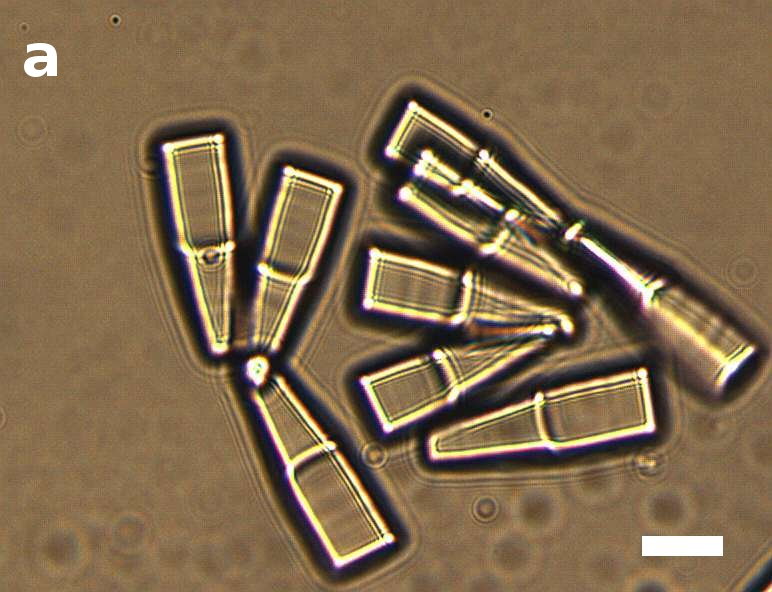
\includegraphics[height=1.5in]{figures/rods/large-janus-rods-45x11x11um.jpg}
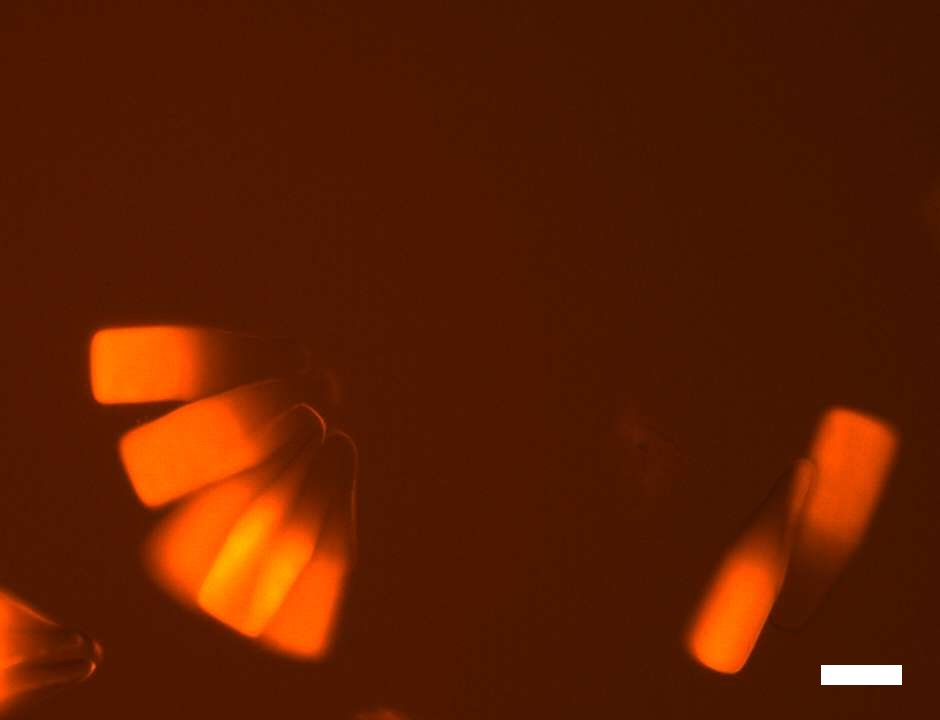
\includegraphics[height=1.5in]{figures/rods/large-janus-self-assembly.jpg}
\end{center}
\caption{Large Janus rods self-assemble following agitation. The hydrophilic 
ends are dyed with Rhodamine B.}
\label{fig:big-janus-assembly}
\end{figure}

Initial hydrophobic/hydrophilic Janus fabrication experiments 
were performed using microchannels fabricated with a height of 15 \microns, 
producing relatively large Janus particles (Figure~\ref{fig:big-janus-high-conc}). These particles had dimensions 
of roughly 45 \by 11 \by 11 \microns, and exhibited little spontaneous self-assembly in water.  However, agitation
of these particles to drive their rearrangement into new configurations produced substantial substantial
self-assembly (Figure~\ref{fig:big-janus-assembly}), producing clustered structures with high contact
areas between the hydrophobic regions of the particles.  This served as a proof-of-concept of 
hydrophobic self-assembly and duplication of the
results from Dendukuri \textit{et al.}~\cite{dendukuri-amph}.  

\begin{figure}
\begin{center}
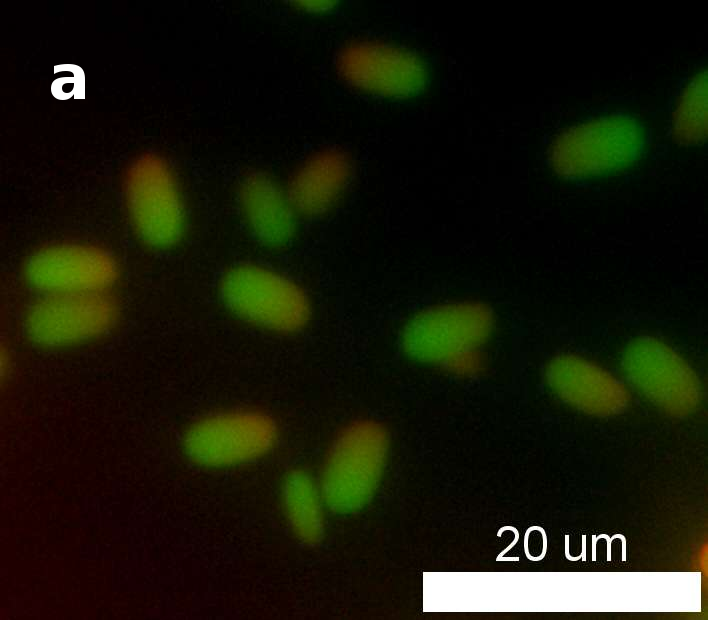
\includegraphics[height=1.5in]{figures/rods/janus-rods-4x2um.png}
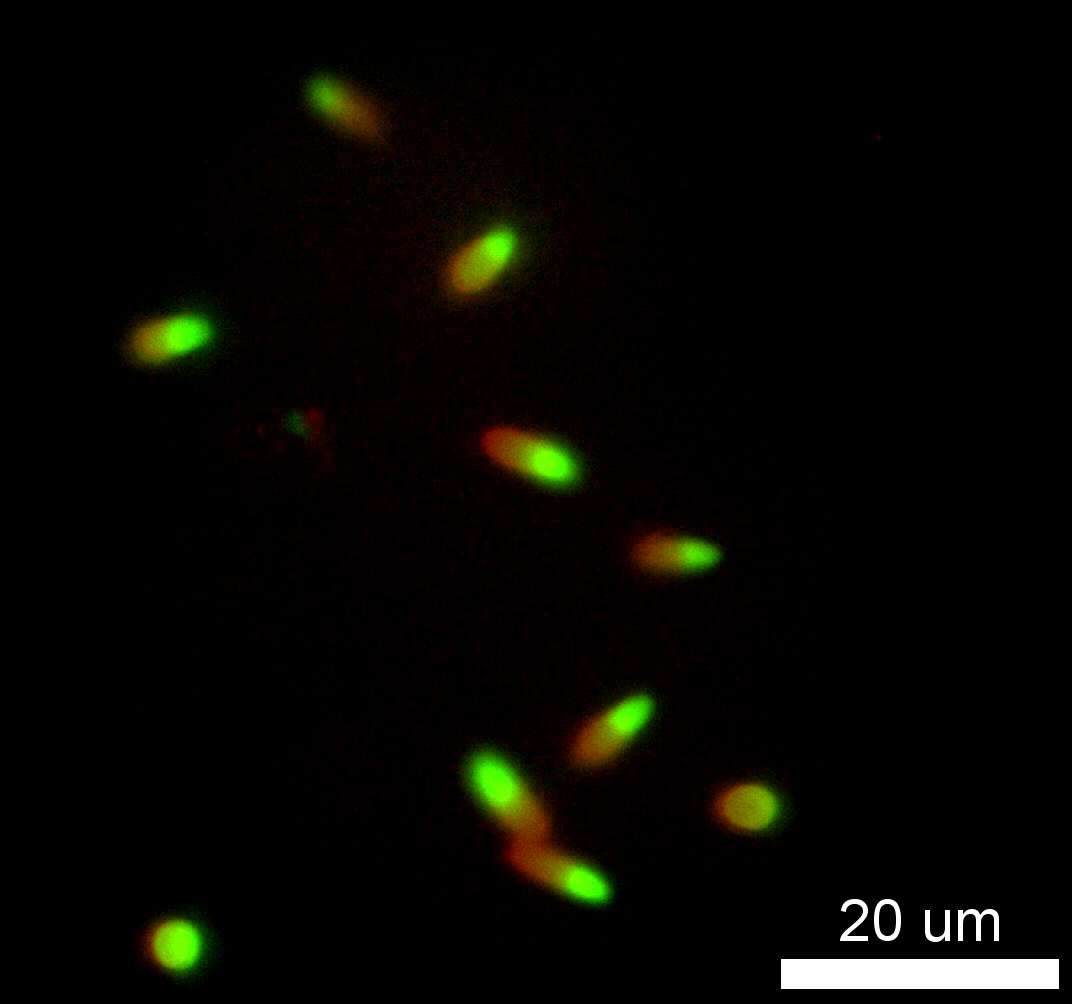
\includegraphics[height=1.5in]{figures/rods/janus-rods-6x2um.png}
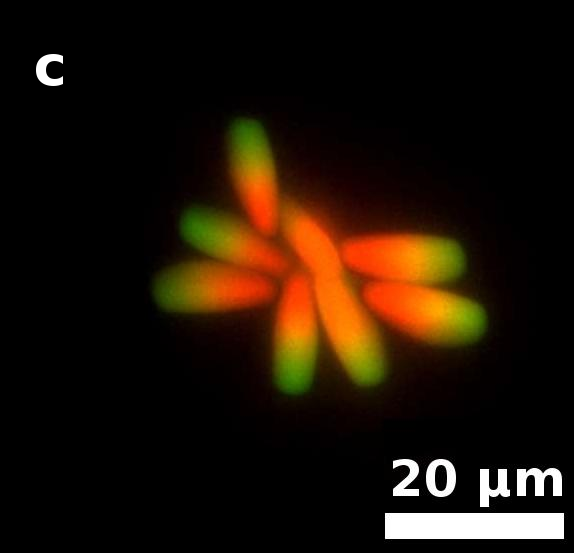
\includegraphics[height=1.5in]{figures/rods/janus-rod-cluster-zoom.png}
\end{center}
\caption{Various sizes of Janus rods.}
\label{fig:janus-sizes}
\end{figure}

Next, the fabrication microchannel was reduced in height to 7 \microns~and the mask size was varied to explore the
size limitations in fabricating Janus rods.  Janus rods were successfully fabricated 
using 500 \microns, 300 \microns~and 200 \microns~masks to produce Janus rods with lengths of 
15 \microns, 7 \microns~and 4 \microns~respectively. (See Figure~\ref{fig:janus-sizes}(a,b,c).)

\figone{fig:assembly-v-solvent}{figures/rods/janus-rod-assembly-vs-solvent.png}{0.8\linewidth}{
Self-assembly of Janus rods in (a) water, (b) DMSO and (c) IPA.}

To explore the effect of assembly solvent on the resulting structures, identical Janus rods with dimensions 
12 \by 3 \by 3 \microns~were fabricated and placed in three different solvents: water, dimethyl sulfoxide 
(DMSO) and isopropyl alcohol (IPA).  In water, we see a result similar to that seen for the large Janus rods,
with strong hydrophobic self-assembly producing structured clusters, with strongly-correlated orientations
between the rods within a cluster.  Suspension and agitation in DMSO, however, shows little or no self-assembly.
This result is consistent with DMSO's status as a less polar solvent than water, decreasing the driving force
for hydrophobic self-assembly.  Moving the particles to IPA, a non-polar solvent, shows a completely different
self-assembly behavior following agitation, in which the green-dyed hydrophilic parts of the particles are 
assembling to maximize contact area.  This series of experiments illustrates the potential for 
control of self-assembly via varying the solvent conditions.

\figone{fig:assembly-small-clusters}{figures/rods/janus-rods-large-clusters-ordered.png}{0.8\linewidth}{
Janus rods self-assemble at low concentrations into small ``micellar'' structures.}

\figone{fig:large-struct}{figures/rods/janus-rods-large-structures.png}{0.8\linewidth}{
Janus rods self-assemble at high concentration into extended, gel-like structures in water.}

Focusing on self-assembly in water, we see that a variety of different structures may be 
achieved.  In a single sample, local variations in concentration due to uneven mixing may produce
dramatically different results.  Where the local concentration is low, highly-ordered clusters 
are produced which have a ``micelle-like'' geometry, with the particles grouped around a common 
center where the hydrophobic regions tend to maximize contact area 
(Figure~\ref{fig:assembly-small-clusters}).  Where the local concentration
is high, however, extended structures containing many more particles may be formed
(Figure~\ref{fig:large-struct}).  These
structures have a ``gel-like'' motif in that they are more randomly arranged, but still contain
sub-clusters which are formed by hydrophobic assembly.

\begin{figure}
\begin{center}
\includegraphics[width=0.5\linewidth]{figures/rods/janus-tiled-large-area.jpg} \\

\vspace{12pt}

\includegraphics[width=0.5\linewidth]{figures/rods/high-conc-large-area.png}
\end{center}
\caption{
A large-area view of Janus rod self-assembly in DMSO/water at a low concentration,
at low and high magnifications.}
\label{fig:large-area}
\end{figure}

\figone{fig:bonds-per-particle}{figures/rods/struct-plot-2.jpg}{0.8\linewidth}{
Bonds per Janus particle.}

\figone{fig:orientation-plot}{figures/rods/struct-plot-1.jpg}{0.8\linewidth}{
Orientational ordering.}

A more quantitative study of Janus rod self-assembly was attempted by fabricating large 
numbers of Janus rods and observing their self-assembly in confocal observation chambers.
Fabrication sample size for each experiment was approximately 50,000 particles; losses
due to transfer and processing reduced this to an estimated 20,000 particles.
Two parameters were varied: the assembly solvent, which was a mixture of DMSO and water
with the relative fraction adjusted; and the aspect ratio of the particle, which was varied
in the range of 1.5-4.5.  Large-area images were acquired as detailed in 
Section~\ref{sec:tiled-microscopy}, and analyzed as detailed in Sections~\ref{sec:rod-tracking}
and~\ref{sec:structure-calcs}.  Sample images at low and high magnification are shown
in Figure~\ref{fig:large-area}.

Two parameters were calculated for each sample: the average number of contacts or ``bonds''
per particle, and the degree of orientational ordering for particles in the same cluster.
The number of ``bonds'' was calculated as the number of particles which were found within a 
center-to-center distance equal to one rod length.  The orientational ordering was measured
as the average dot-product of the orientation vectors between pairs of rods which were 
considered to be in the same cluster, with clusters defined according to the same bond criterion.
The results of these calculations are plotted for all experiments in Figures~\ref{fig:bonds-per-particle}
and~\ref{fig:orientation-plot}.  Unfortunately these results are somewhat contradictory, and it 
is difficult to draw good conclusions about the behavior of Janus rods undergoing self-assembly;
but it is possible to make a few general comments.

The first thing that should be noted is that for all experiments, the average number of bonds per
particle never exceeds about 0.6, and in fact most experiments have bond numbers below 0.2.  This
can be attributed to the fact that despite the high number of particles fabricated relative to
typical SFL experiments, the rod concentrations are still quite low: settled to the bottom of the
container, the average areal concentration never exceeds about 5\%.  The bond numbers for 
DMSO/water mixtures of 50--100\% water are all relatively similar, in the range of 0.1--0.2, and do
not vary much with aspect ratio.  

For solutions with greater than 
50\% DMSO, however, we see a striking increase in bond number.  Without carrying out additional experiments it 
is difficult to determine the cause of this increase. We might speculate that the higher density of DMSO
and the consequent slower settling might allow the rods more time to ``find'' one another and assemble, but in
this case we would expect a more continuous variation of bond number with DMSO concentration. Another cause might
be some experimental error which increased the final particle yield in the high-DMSO samples relative to the others.
Within these samples, however, we see a consistent variation in bond number with respect to aspect ratio, with
much higher bond numbers observed at low and high aspect ratios.  The increase in bond number at low aspect ratio, 
and thus low particle size, might be attributed to the higher mobility of these particles on a surface where
Janus particles would tend to stick (see Section~\ref{sec:surface-interact}), while the increase at high aspect
ratio may be due to the higher opportunity for contact available with longer rods.

Turning our attention to the orientational ordering, we see much more consistent results across the
range of solvent compositions, with little in the way of consistent discernible variation between samples with
the same aspect ratio.  A dot-product of 1.0 implies perfect parallel ordering, while a dot product of 0.0 implies
perpendicular ordering; average values close to 0.5 may be interpreted as showing relatively random orientation
within the sample.  With that in mind, it is interesting to note that particles with low aspect ratio show 
a relatively strong ordering, and that the dot product decreases towards randomness as the aspect ratio 
increases.  This is somewhat counter-intuitive, and contradicts some previous imaging which would suggest
better correlation between particles with a high aspect ratio.

%%%%%%%%%%%%%%%%%%%%%%%%%%%%%%%%%%%%%%%%%%%%%%%%%%%%%%%%%%%%%%%%%%%%%%%%%%%%%%%%%%%%
\subsection{Potential Applications}

\begin{figure}
\begin{center}

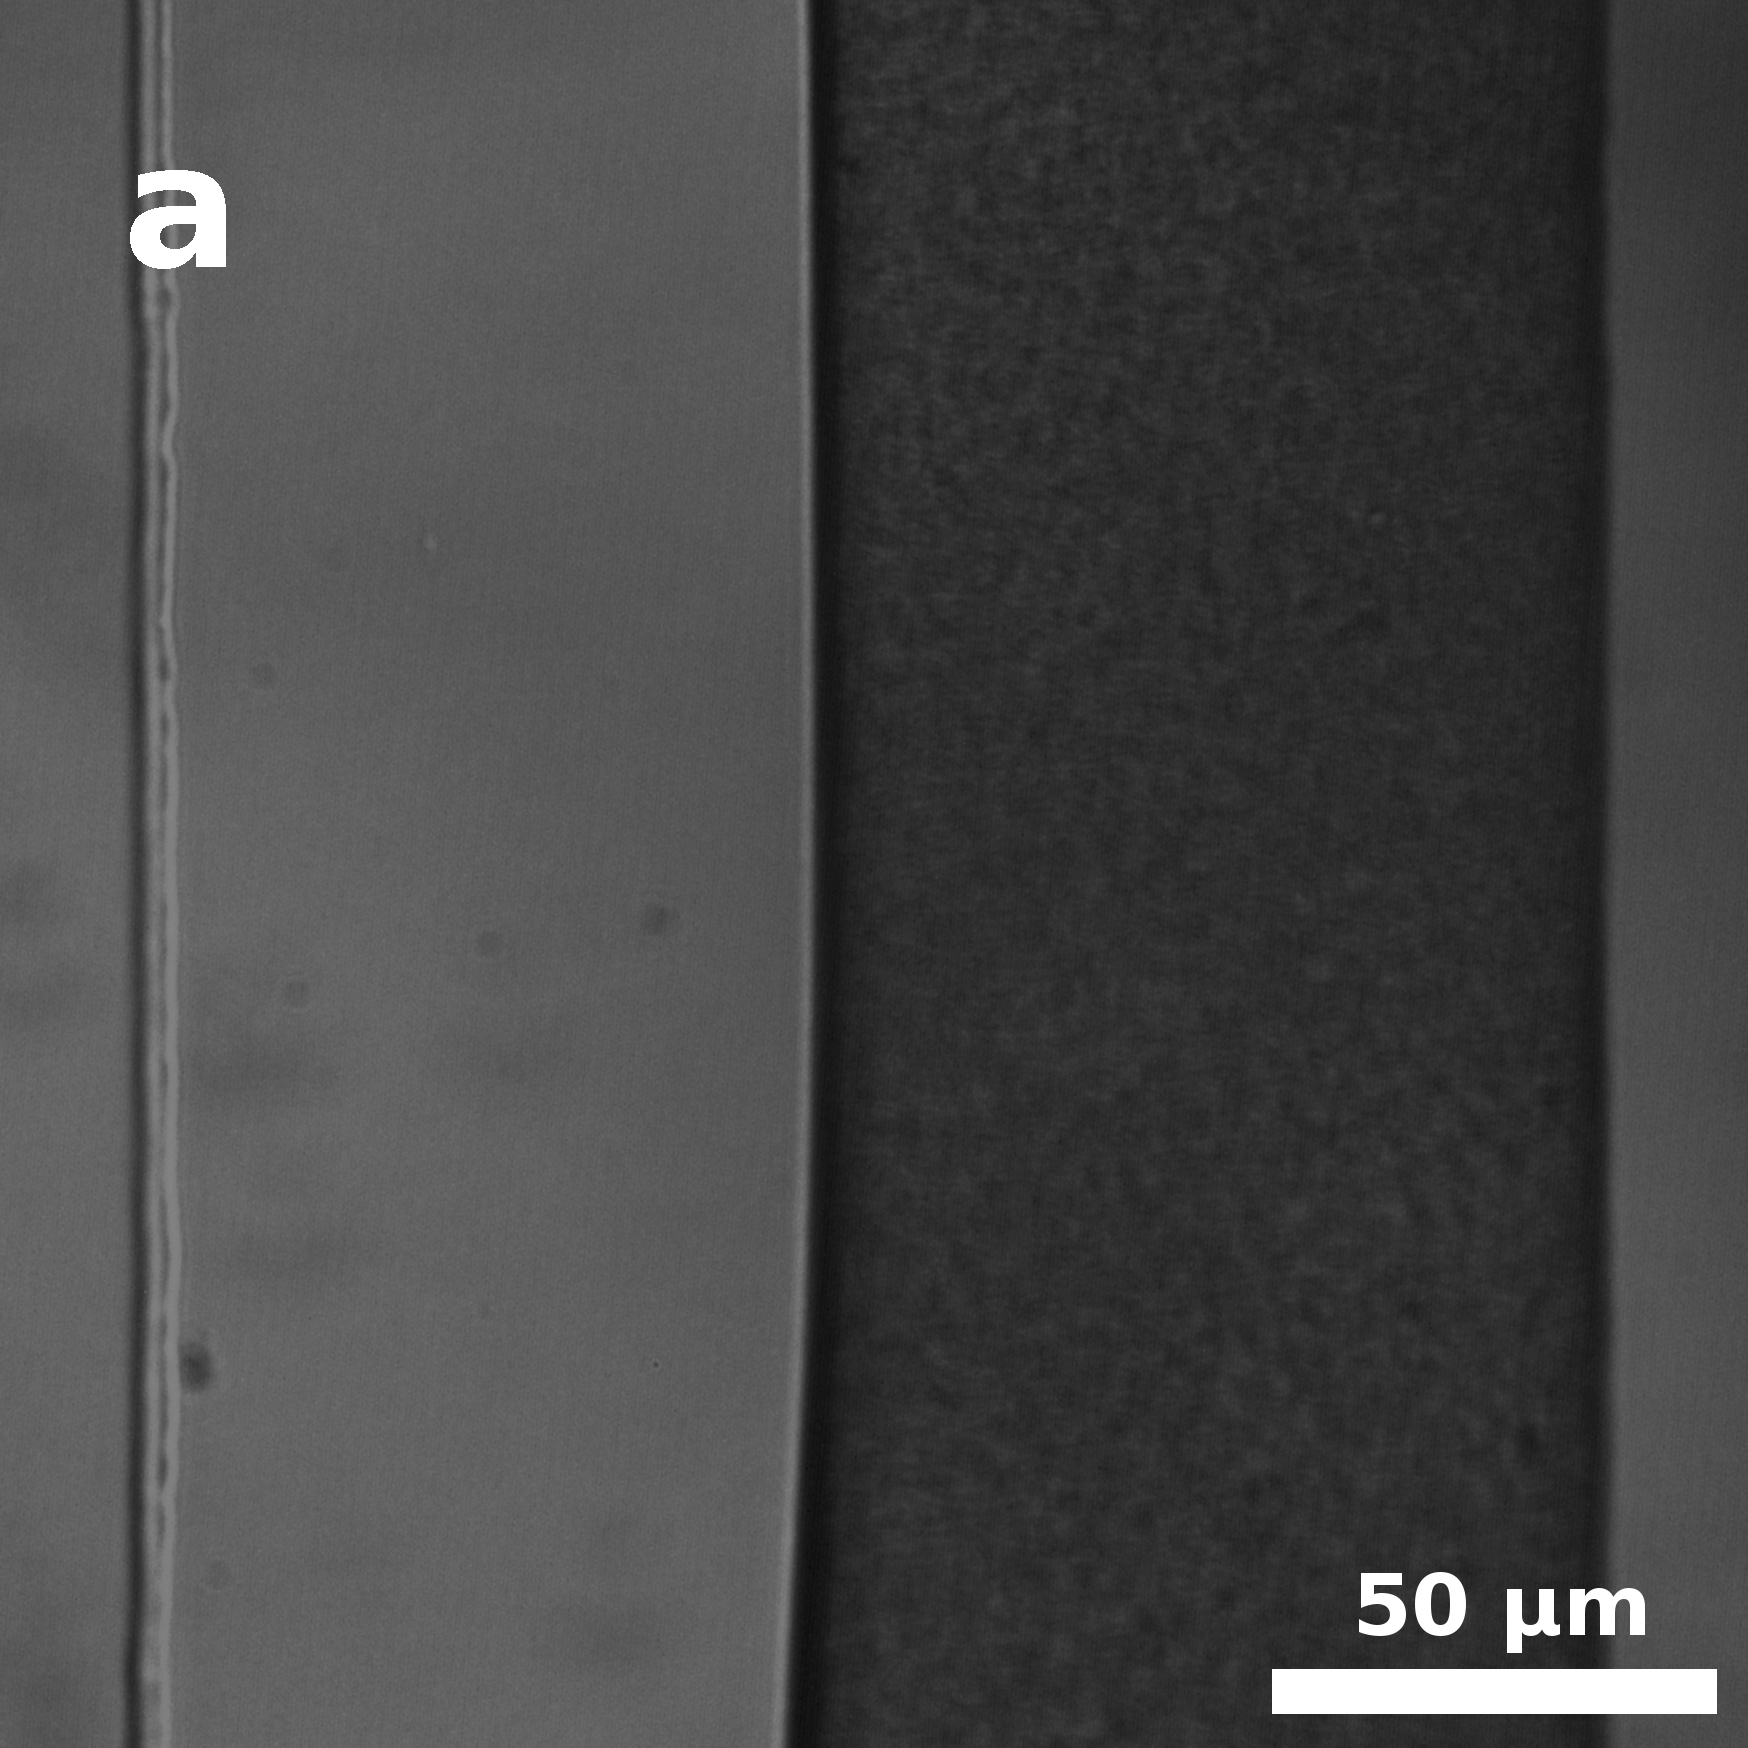
\includegraphics[height=2.5in]{figures/rods/silver-microchannel-twostream.png}
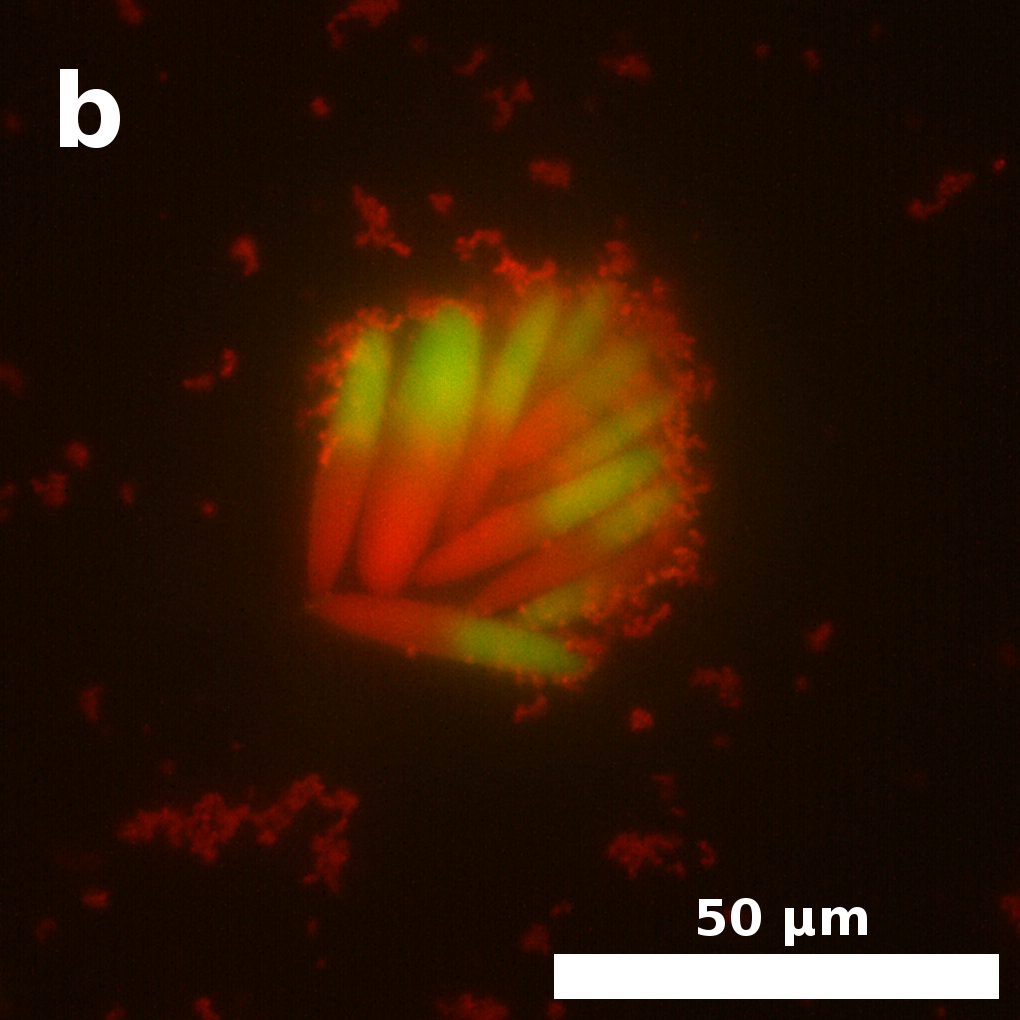
\includegraphics[height=2.5in]{figures/rods/silver-fluorescence-assembly.png}
\end{center}
\caption{
(a) Ag nanoparticles are suspended in PEGDA monomer solution for Janus SFL fabrication, and
(b) Ag nanoparticles are embedded in at 5 wt\% in otherwise-standard PEGDA monomer solution, and Janus rods
are fabricated as a demonstration of self-assembled functional Janus rods.}
\label{fig:silver-janus}
\end{figure}

The potential for the incorporation of functional materials into SFL Janus particles was 
explored in a pilot experiment involving the incorporation of Ag nanoparticles (NPs) into the
hydrophilic PEGDA monomer solution at 5 wt\%. A Janus fabrication experiment using this 
solution was set up, and the Ag NPs were shown not to interfere with the establishment of a stable
pair of co-flowing streams (see Figure~\ref{fig:silver-janus}(a)). Standard Janus SFL was carried
out using a 400 \microns~mask to produce 12 \microns~Janus rods. When placed in water, these rods
self-assembled normally, as shown in Figure~\ref{fig:silver-janus}(b).  Note, however, the presence of
free Ag NPs (fluorescing red) both in the free solution and aggregated around the assembled cluster.
This illustrates a major difficulty in incorporating any functional material in SFL, i.e. the successful 
rinsing and removal of functional materials from the suspension solvent.

